% !TEX root = ../elsarticle-template.tex
%-------------------
\section{Case Study: The VaryMDE Project}
\label{sec:validation}

In this section, we introduce the VaryMDE project which is bilateral collaboration between INRIA and Thales Research \& Technology (TRT). The role of this project in the research presented in this article is two-fold. On one hand, it provides a set of research questions that motivate our work. Concretely, the research presented in this article represents an answer to some of the needs emerging in Thales in terms of language engineering. On the other hand, this project provides a realistic application scenario which we used as validation of the approach. In the reminder of this section, we present an overview of the project and we discuss the results of applying our approach in the scenario introduced by Thales.  

%INRIA' Diverse team worked togueter with Thales Research \& Technology (TRT) researchers towards targueting variability management issues at both the modeling level and the metamodeling level (i.e., design and implementation of software languages). Concretely, Thales researchers ended up having DSLs defined using three finite-state machines specifications and needed supoprt to avoid future costs. In the Section \label{sec:validation} we present more details about the used case.

 %To evaluate of our approach, we use a set of DSLs for state machines. Note that a simplified version have been used as running example along this paper (see Section \ref{sec:thedevelopmentscenario}). This scenario is inspired from the analysis of variability on languages for finite state machines provided by Crane et al. \cite{Crane:2007}, and it is composed of three different DSLs: UML state diagrams, Rhapsody, and Harel's state charts. As aforementioned, these DSLs have some commonalities since they are intended to express the same formalism. According to the development scenario we address in this paper, these commonalities will be materialized as clones in the DSL specifications. In this section, we summarize both commonalities and differences existing in the case study. Then, we apply our approach and we present the obtained results. To explain this scenario we try to follow as close as possible the guidelines provided by \cite{runeson-book} for the sake of clarity and organization. Note that we do not claim this to be a case study.

\subsection{Background to the research project}
Thales is a company whose business model turns around the construction of different types of systems that solve needs in diverse domains such as transport, aerospace, security, or defense. During the construction of these systems, Thales' engineers often appeal to the use of state machine languages to express behavior.

Despite the expressibility of state machines, the diversity of the systems built by Thales imposes an accidental complexity. Depending on the type of system under construction, there are different requirements on the way in which a state machine should be executed. Hence, there is certain semantic flexibility that state machine languages should offer to support the particularities of the systems unde construction. As a result, Thales engineers are intended to build not only the devices themselves but also to adapt the state machines formalisms. 

The typical development process to address the implementation of the formalisms for state machines is as follows: at the beginning, language designers build an initial DSL for state machines that fits the needs of one type of system. Then, they create new development branches when they adapt the first variant of the DSL to the needs of other types of systems. After some repetitions, language designers have a family of DSLs for state machines. Those DSLs have both syntax and semantic differences. 

\subsection{Design of the case study}

\textbf{Objectives.} One of the challenges of the VaryMDE project is to find out a way to facilitate the development process descrived above. As an answer of this challenge, we propose the use of reverse engineering techniques to create language product lines of DSLs for state machines from existing variants.

\vspace{2mm}
\textbf{Planning.} The case study was planned in three phases as shown in Fig. \ref{fig:planning}. In the first phase, the data set is prepared. Such a data set corresponds to the set of DSL variants that will be used to reverse engineer the language product line. This phase is iterative since we need to consider the feedback comming from the Thales' engineers. During the second phase, we execute our approach using the initial set of DSL variants. Finally, in the third phase we analyse the produced language product lines. 

\begin{figure}[h!]
	\centering
	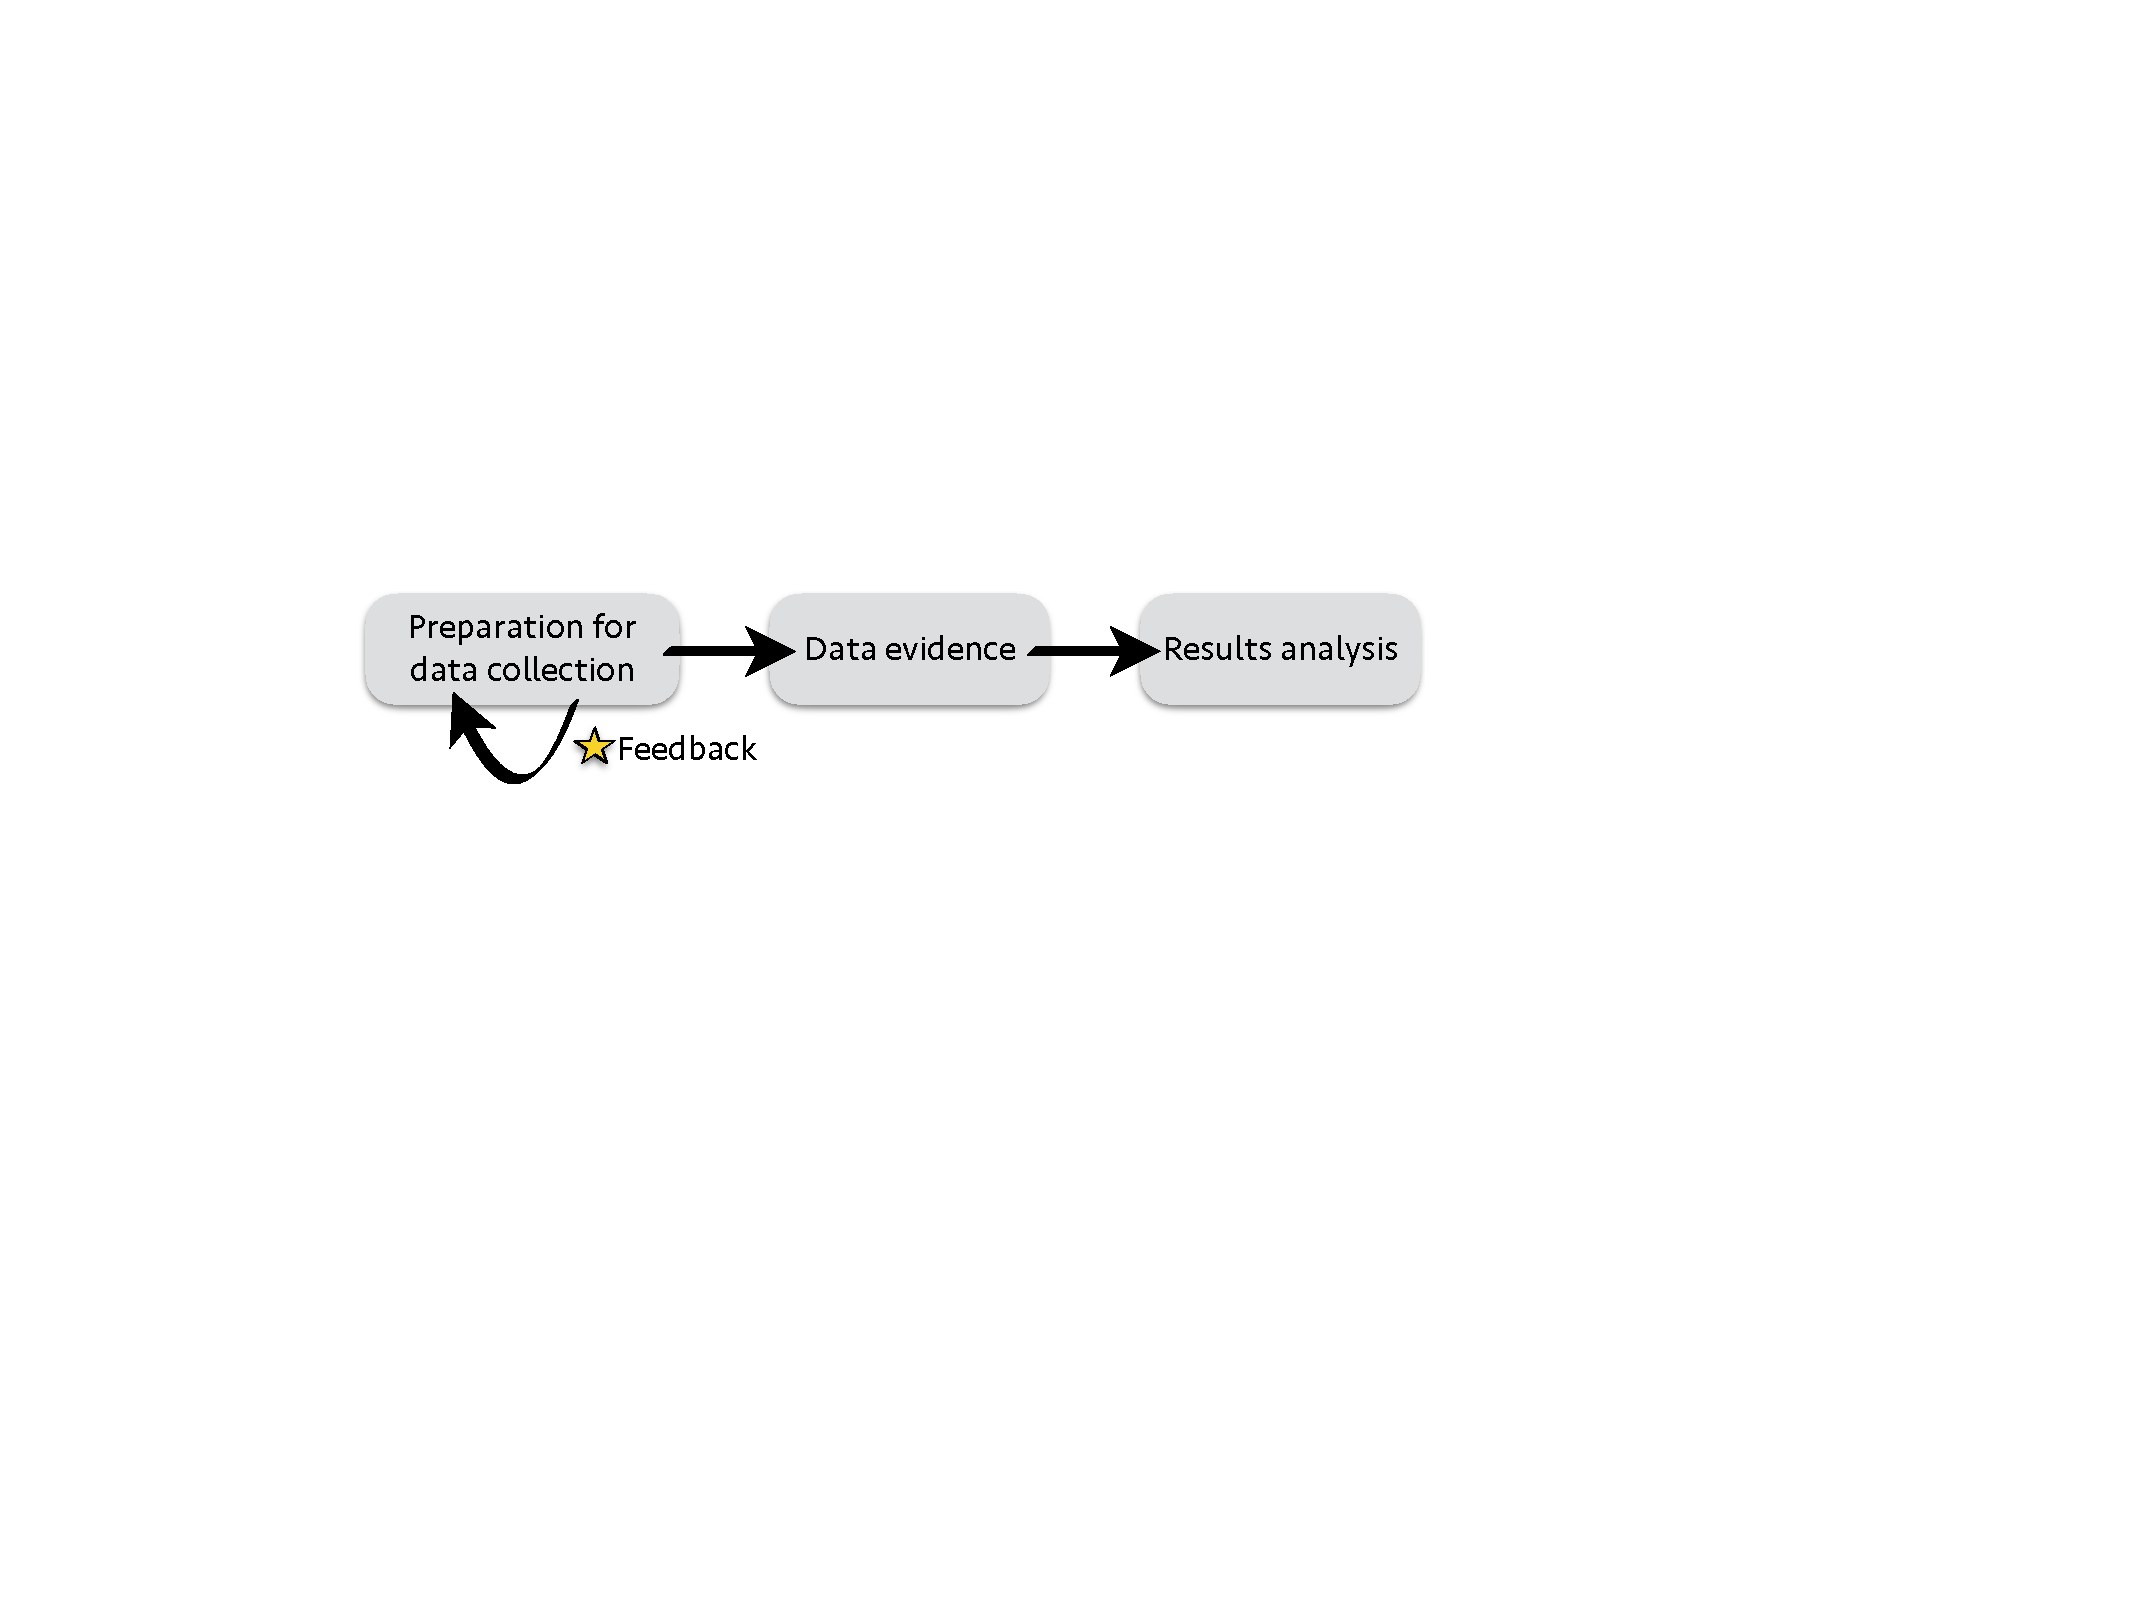
\includegraphics[width=1\linewidth]{images/planning-casestudy-fig.pdf}
	\caption{Planning of the case study}
	\label{fig:planning}
\end{figure}

\subsection{Preparation for data collection}

As aformentioned, the objective in this phase is to define the set of initial DSL variants that will be used to execute our approach. The most important limitation we found at this stage is that many of the implementations for state machine DSLs are built in different language workbenches and using diverse language meta-languages. Under these conditions, commonalities and particularities of DSLs are more difficult to detect.

To overcome such a limitation, we decided to implement the initial DSL variants in a unified language workbench and using the same meta-languages. Hence, the phase of preparation for data collection corresponds to a language development process where three different formalisms for state machiens were implemented: UML state machines, Rhapsody, and Harel statecharts. Those formalisms were selected because they have a complete documentation that allow to fully understand its semantics. The implementation of the formalisms was conducted on top of Melange \cite{Degueule:2015a} language workbench and it is available on a dedicated GitHub repository\footnote{GitHub repository: \url{https://github.com/damende/puzzle/tree/master/examples/state-machines}}. The description of commonalities and differences existing among the selected formalisms are well-studied by Crane et al and are described in Annexe A. 

\subsection{Collecting evidence}

Once we built the initial set of DSLs variants, we execute our approach and obtained a language product line for state machines. The results are summarized in Fig. \ref{fig:results-casestudy}. At the left of the figure we present the set of language modules we obtained as well as the language interfaces existing among them. Those modules group the language constructs according to the heuristic introduced in Section \ref{sec:reverseengineeringmodules} on breaking down intersections. At the right of the figure we show the corresponding variability models. Each feature of the feature models is associated to a given language module. In turn, the semantic variability points in the orthogonal model are associated to clusters of domain specific actions.

%Note that we marked different configurations in the figure to identify each of the corresponding DSLs. In addition, we calculated the number of possible configurations. We obtained that with this variability model, we can obtain XXX DSLs for state machines.

\begin{figure*}
	\centering
	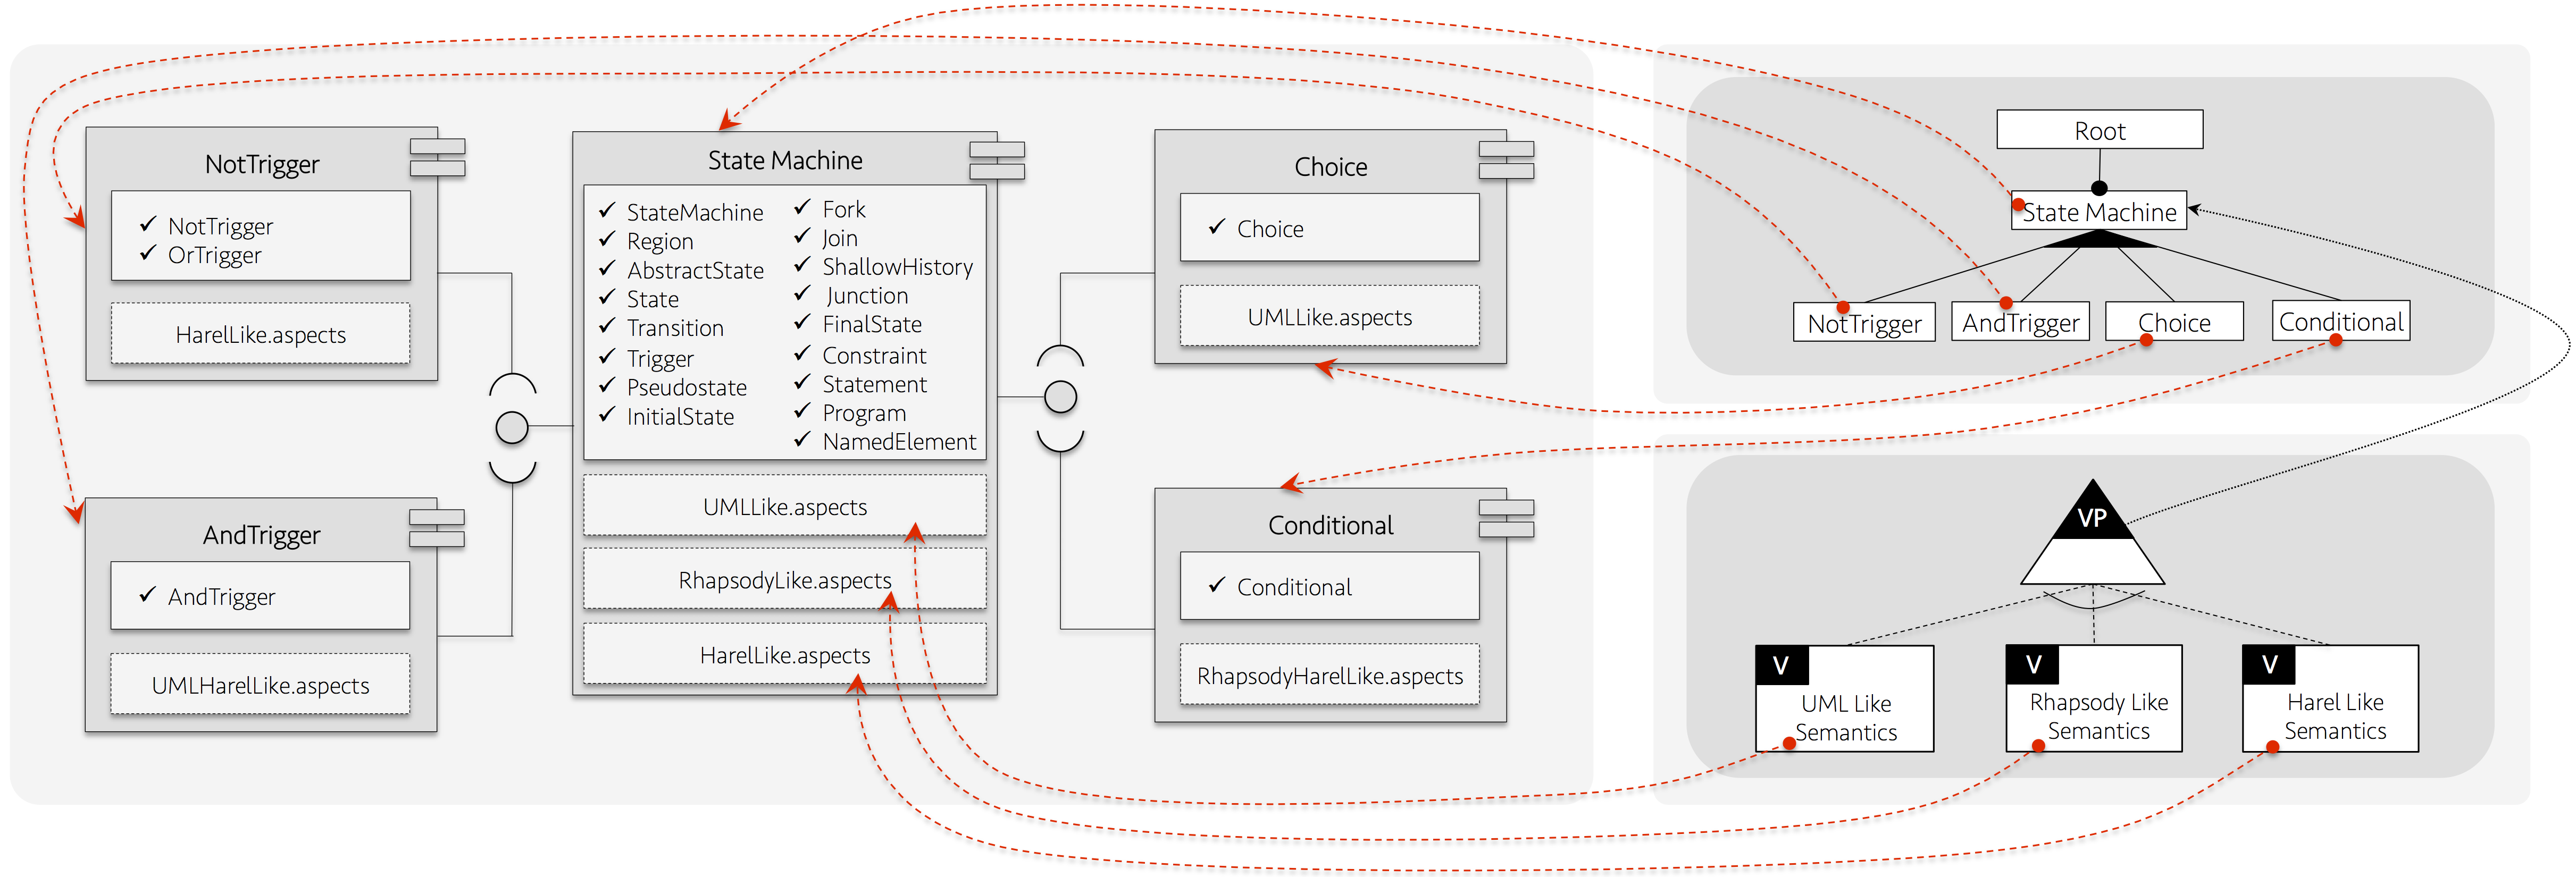
\includegraphics[width=1\linewidth]{images/results-casestudy.png}
	\caption{Language product line produced for the case study of the finite state machines. }
	\label{fig:results-casestudy}
\end{figure*}

\subsection{Analysis of collected data}

Let us now discuss the results of the case study. As expected, we obtained a language product product line from a set of DSL variants for finite state machines. But... Does this product line identify all the variation points and commonalities existing in the DSL variants? Are those variation points properly specified in the language modular design and variability models? Since we know these variation points and commonalities, we can check whether they are appear in the produced language product line. The results of this verification are presented in Table \ref{fig:validation-results}.

The results are promising in the case of abstract syntax variability. According to the Table \ref{fig:oracle}, the DSL variants share 17 constructs in common. Those constructs are properly factorized in a language module that we named StateMachine. This module is correctly identified during the recovering of the language modular design, and it is properly specified as a language module in terms of a metamodel enhance with domain specific actions and offering a provided interface. Besides, the particularities of the DSL variants are also well factorized. There is a module that contains the constructs NotTrigger and OrTrigger that belong only to the variant complying the Harel' statecharts specification. Besides, there are three additional modules that contain the constructs AndTrigger, Choice, and Conditional respectively. Using this modular design, we can re-compose any of the three initial DSL variants.

The situation is different for the case of semantic variability. Although our reverse-engineering strategy is able to identify that the domain specific actions are different in the three DSL variants, the level of granularity at which those variation points are detected is coarser than one might expect. At the beginning of this section, we described three semantic variation points and their possible interpretations i.e., events dispatching policy, execution order of transitions' effects, and priorities of conflicting transitions. Using the proposed technique, we can identify just one semantic variation point indicating that the language module called StateMachines contains three different clusters of domain specific actions, which is reflected in the orthogonal variability model.

This threat to validity of our technique can be explained by the fact that the analysis of commonalities and variability is conducted by means of static analysis. We can analyze the structure of the metamodels and the domain specific actions, but not their behavior at runtime. Hence, we cannot see how these differences impact the execution of the models. For example, we cannot infer that the differences among the domain specific actions in the StateMachine module impact the way in which conflicting priorities are managed. A next step in this research could be to use also dynamic analysis in the domain specific actions to better specify semantic variation points.

\begin{table}
\centering
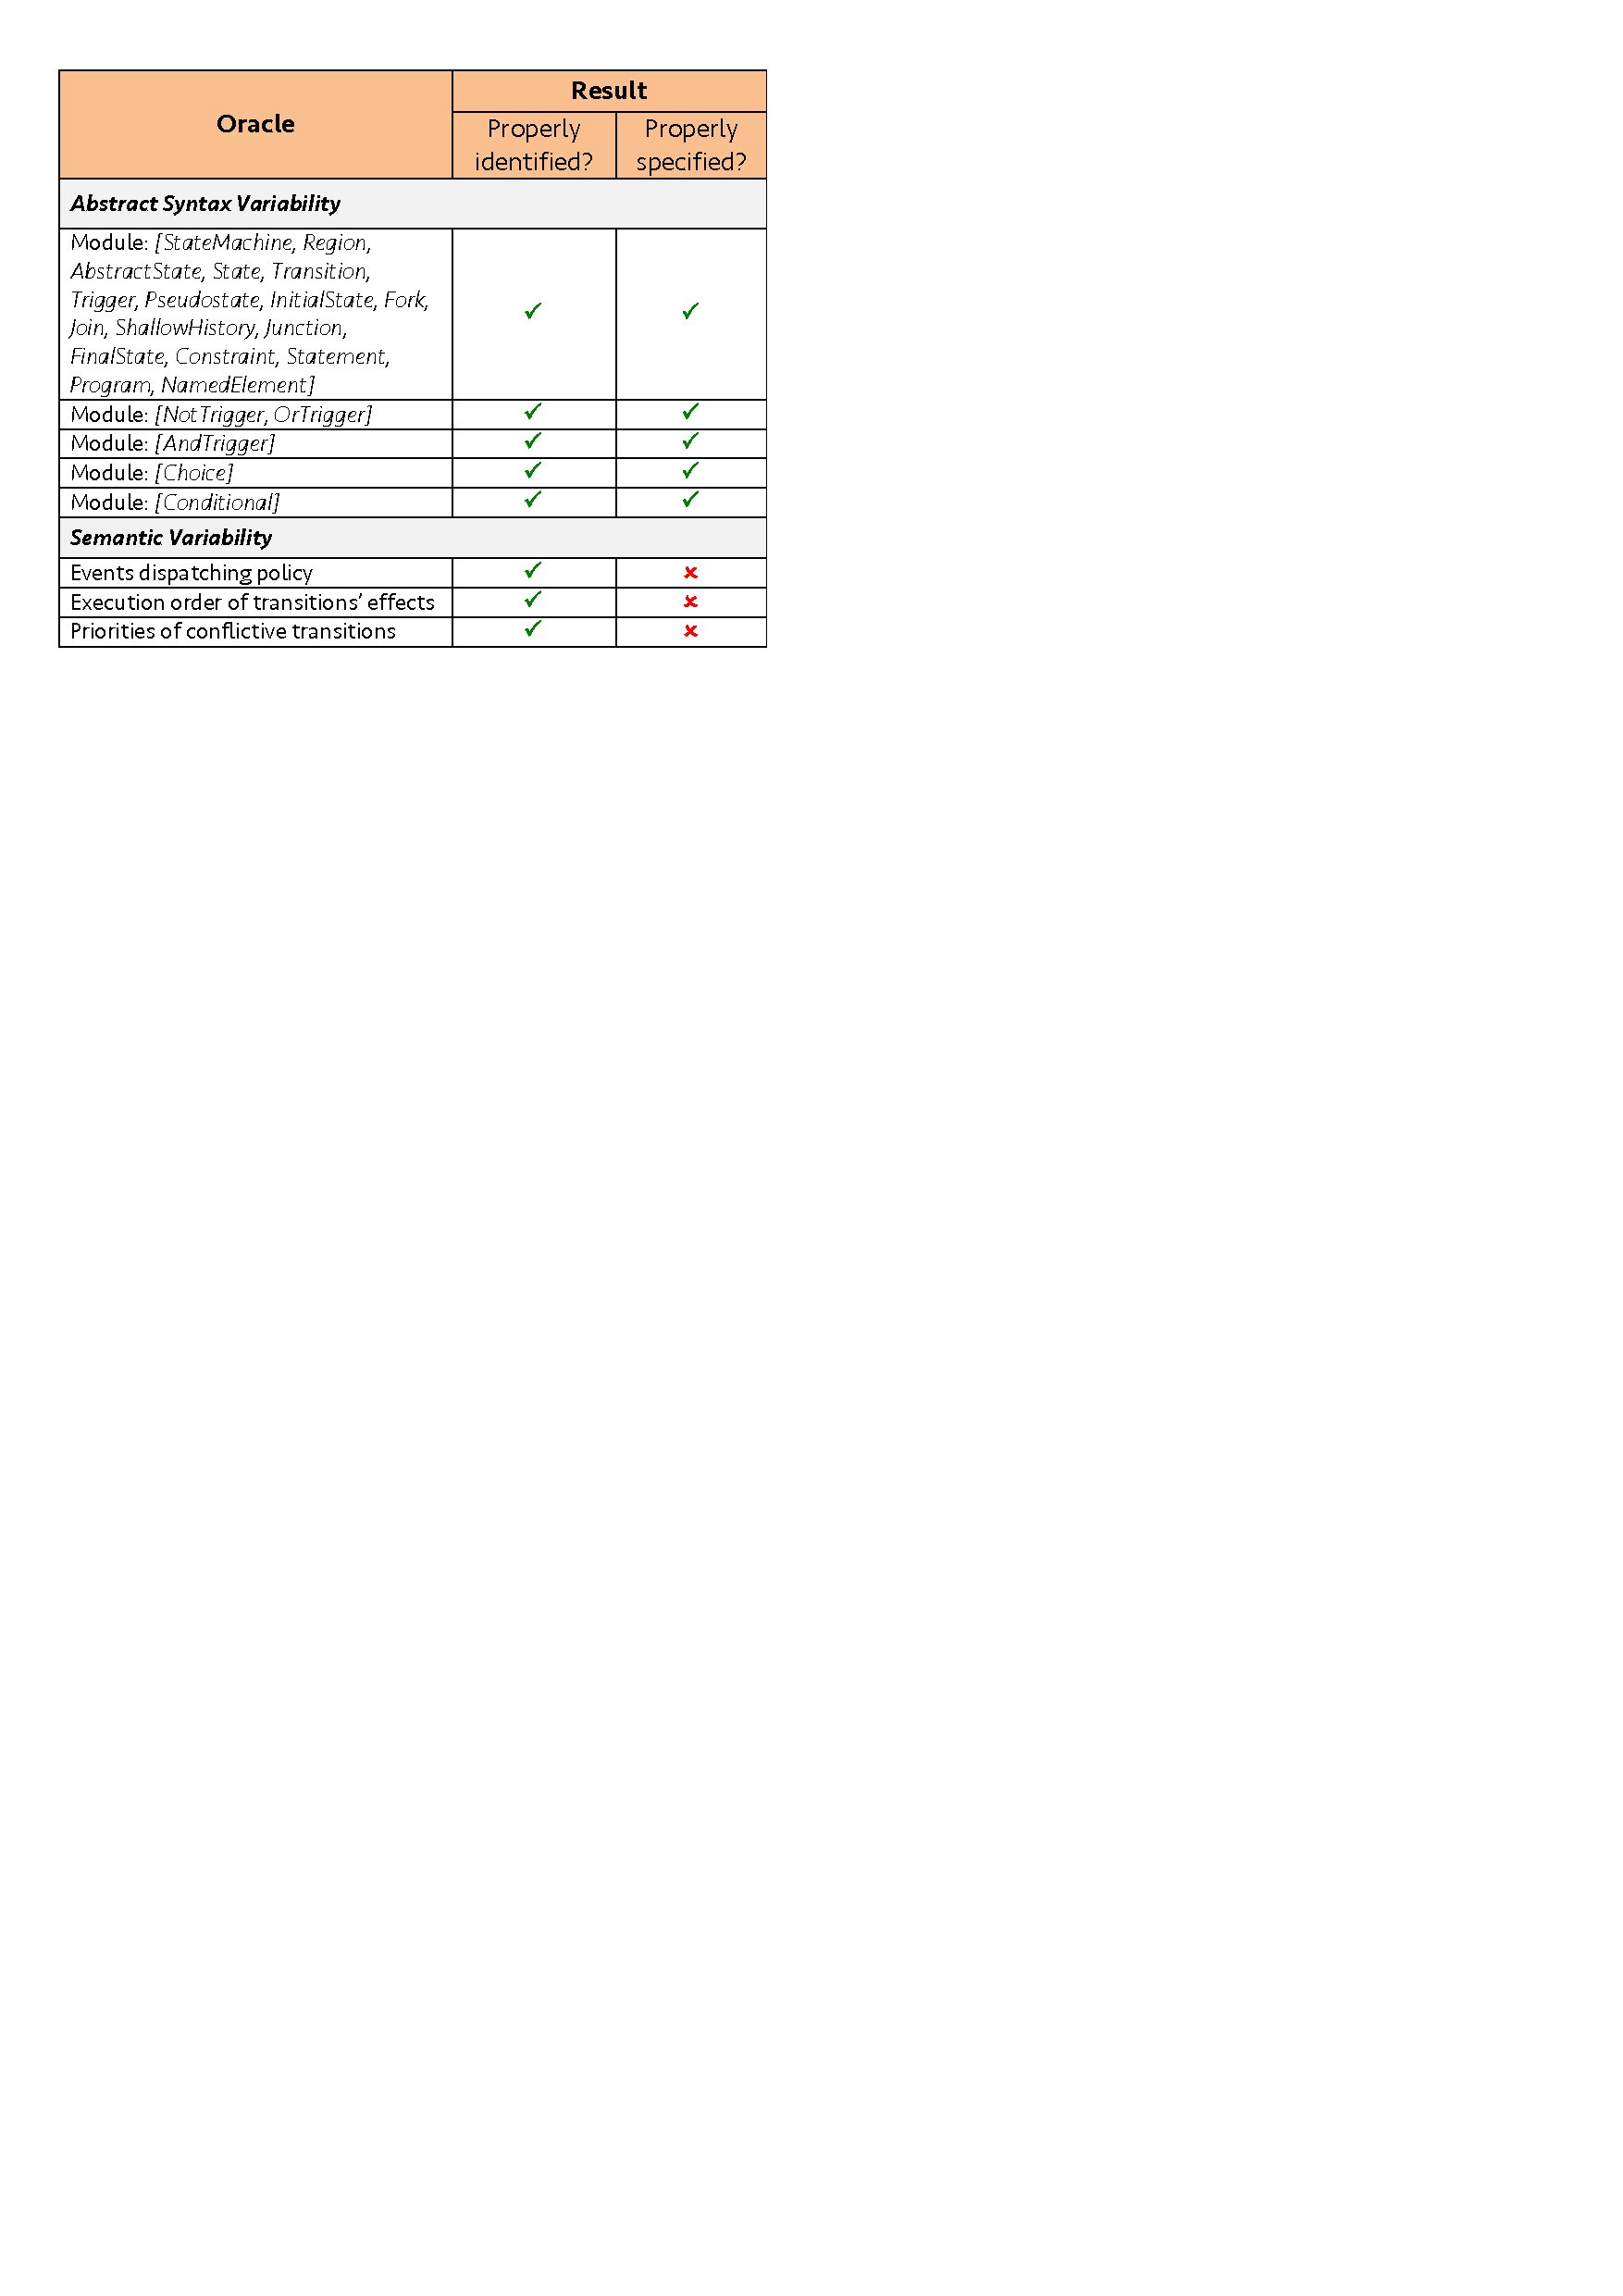
\includegraphics[width=1\linewidth]{images/validation-results}
\caption{Analysis of the results of the case study}
\label{fig:validation-results}
\end{table}

%\subsubsection{Units of Analyses}
%Three different formalims were considered i) UML; ii) Rhapsody, and; iii) Harel's statecharts. For each of take a look to two properties of them. First, the commonalities, this is the common parts to all the existing state machines formalisms. Second, the variabilities or the parts that differ between the different formalims.

%\paragraph{Methods, data collection and measures}
%The main source of information in this enquiry is the set of meetings that some of the authors had with the representative of the Thales side of the project. A total of \todo[inline]{XX} meetings were held. After the first one a set of software artifacts were provided for a detailed analysis as well as the requisites for each formalism.

%The data were collected in the following ways

%\begin{itemize}
%	\item Artifacts analysis, we received from Thales a set of models and metamodels depicting the diferent state machines that the thales group uses.
%	\item Interviews, we performed several meeting to ask for the aplications and plans for the metamodels and its variabilities and commonalities.
%\end{itemize}